\documentclass{article}[12pt]
\usepackage[left = 15mm, right = 15mm, top = 0.25in, bottom = 0.25in, a4paper, inner=1.5cm, outer=3cm, top=2cm,
bottom=3cm, bindingoffset=1cm] {geometry}
\usepackage[utf8]{inputenc}
\usepackage[T5]{fontenc}
\usepackage{lipsum}%to generate dummy data
\usepackage{times}
\usepackage{graphics}
\usepackage{diagbox}
\usepackage{float}
\title{\fontsize{17.5pt}{18.5pt}\selectfont Bài 12: Xác định tốc độ ánh sáng - Lớp 65MNEC}
\author{\fontsize{17.5pt}{18.5pt}\selectfont Đỗ Đức Tiến}
\date{\fontsize{17.5pt}{18.5pt}\selectfont Ngày 1 tháng 6 năm 2022}

\begin{document}
	\maketitle
	\section{\fontsize{17.5pt}{18.5pt}\selectfont Mục đích thí nghiệm}
	 \fontsize{13.5pt}{14.5pt}\selectfont Nghiên cứu cách đo vận tốc ánh sáng bằng phương pháp quang điện trên dao động ký điện tử.
	\section{\fontsize{17.5pt}{18.5pt}\selectfont Cơ sở lý thuyết}
	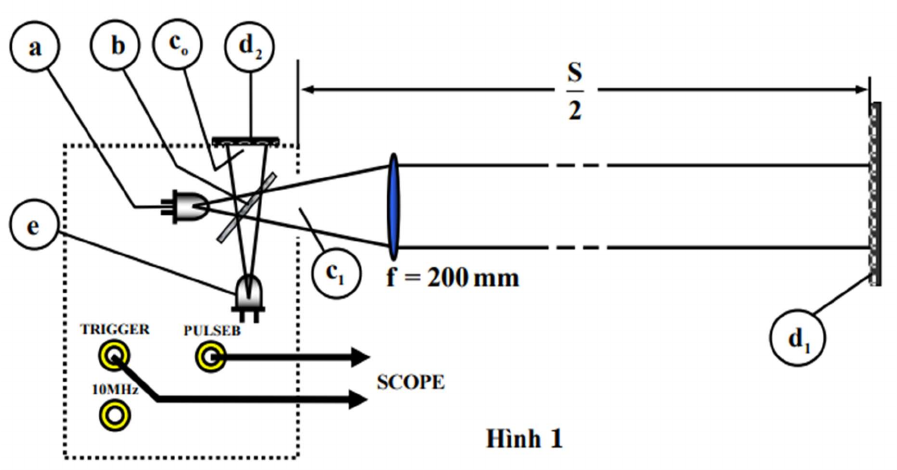
\includegraphics{download.png}
	\begin{itemize}
		\item Xác định vị trí của đèn LED nuôi ở nguồn xung vuông rồi hình thành các chớp sáng. Sau đó chúng ta sẽ đặt gương d1 với khoảng cách S/2. Chùm sáng đo sau khi phản xạ từ gương (d1), lại qua gương bán mạ (b) tới điốt quang - điện (e) (điốt quang - điện (e) là một Sensor biến đổi tín hiệu quang thành tín hiệu điện). Mỗi một thay đổi của xung ánh sáng, sau khi đi qua quãng đường S, làm xuất hiện trên dao động kí một hiệu điện thế xung gọi là tín hiệu thời gian đo (U1)
		\item Nếu cho gương (d1) dịch chuyển một đoạn S/2 thì quãng đường ánh sáng đi được thay đổi một đoạn \makebox[0.5cm]{\[\Delta S\]} , tín hiệu thời gian U1 trên dao động kí sẽ thay đổi là t . Vận tốc ánh sáng có thể xác định từ độ dốc của đồ thị hàm số\makebox[2.75cm]{$$\Delta S\ = f\Delta t $$}bằng cách ghi lại những cặp giá trị tương ứng.
	\end{itemize}
	\section{\fontsize{17.5pt}{18.5pt}\selectfont Số liệu}
	Ta có số liệu đo được ở bảng dưới đây:\\
	Bảng 1:
	\begin{table}[H]\centering\setlength\tabcolsep{12.5pt}\renewcommand\arraystretch{1.25}
		\noindent\makebox[\textwidth]{%
			\begin{tabular}{|l|*{3}{c|}}
				\hline
				\diagbox[width=\dimexpr \textwidth/8+2\tabcolsep\relax, height=1cm]{STT}{S(m)}
				& 14 & 18 & 22 \\
				\hline
				1 & 44.8& 58.0 & 69.5 \\
				\hline
				2 & 44.5 & 60.0 & 71.4 \\
				\hline 3 & 44.0 & 61.0 & 70.1\\
				\hline
				4 & 46.0& 60.6 & 71.8 \\
				\hline
				5 & 45.0 & 59.5 & 72.0 \\
				\hline
				\[\overline t  + \overline {\Delta t} (s)\]  & \[44.86 \pm 0.51\] &\[59.82 \pm 0.86\]& \[70.96 \pm 0.93\] \\
				\hline
			\end{tabular}
		}%
	\end{table}
	Bảng 2:
	\begin{table}[H]\centering\setlength\tabcolsep{12.5pt}\renewcommand\arraystretch{1.25}
		\noindent\makebox[\textwidth]{%
			\begin{tabular}{|l|*{3}{c|}}
				\hline
				\diagbox[width=\dimexpr \textwidth/8+2\tabcolsep\relax, height=1cm]{STT}{S(m)}
				& 4 & 8 & 12 \\
				\hline
				1 & 14.3 & 26.1 & 40.5 \\
				\hline
				2 & 15.1 & 27.3 & 41.8 \\
				\hline 3 & 12.9 & 28.0 & 42.1\\
				\hline
				4 & 14.8 & 25.8 & 40.0 \\
				\hline
				5 & 16.0 & 28.8 & 39.5 \\
				\hline
				\[\overline t  + \overline {\Delta t} (s) \]  & \[14.62 \pm 0.82\] &\[27.20 \pm 1.00\]& \[40.78 \pm 0.94\] \\
				\hline
			\end{tabular}
		}%
	\end{table}
	\section{\fontsize{17.5pt}{18.5pt}\selectfont Xử lý số liệu}
	\subsection{Giá trị vận tốc}
	Từ số liệu ở Bảng 1: \\
	\begin{itemize}
	    \item Ta có: \makebox[2.5cm]{\[{S_1} = 14(m)\]}
	    \[{\delta _1} = \frac{{\overline {\Delta {c_1}} }}{{\overline {{c_1}} }} = \frac{{\overline {\Delta {t_1}} }}{{\overline {{t_1}} }} = \frac{{0.51}}{{44.86}} \approx 0.011\]
	    \[\overline {{c_1}}  = \frac{{{s_1}}}{{\overline {{t_1}} }} = \frac{{14}}{{44.86*{{10}^{ - 9}}}} = 3.12*{10^8}(m/s)\]
	    \[ \Rightarrow \Delta {c_1} = \delta *\overline {{c_1}}  = 0.34*{10^8}(m/s)\]
	    \[ \Rightarrow {c_1} = (3.12 \pm 0.34)*{10^8}\left( {m/s} \right)\]
	    \item Ta có: \makebox[2.5cm]{\[{S_2} = 18(m)\]}
	    \[{\delta _2} = \frac{{\overline {\Delta {c_2}} }}{{\overline {{c_2}} }} = \frac{{\overline {\Delta {t_2}} }}{{\overline {{t_2}} }} = \frac{{0.86}}{{59.82}} \approx 0.014\]
	    \[\overline {{c_2}}  = \frac{{{s_2}}}{{\overline {{t_2}} }} = \frac{{18}}{{59.82*{{10}^{ - 9}}}} = 3.01*{10^8}(m/s)\]
	    \[ \Rightarrow \Delta {c_2} = \delta *\overline {{c_2}}  = 0.042*{10^8}(m/s)\]
	    \[ \Rightarrow {c_2} = (3.01 \pm 0.04)*{10^8}\left( {m/s} \right)\]
	    \item Ta có: \makebox[2.5cm]{\[{S_3} = 22(m)\]}
	    \[{\delta _3} = \frac{{\overline {\Delta {c_3}} }}{{\overline {{c_3}} }} = \frac{{\overline {\Delta {t_3}} }}{{\overline {{t_3}} }} = \frac{{0.93}}{{70.96}} \approx 0.013\]
	    \[\overline {{c_3}}  = \frac{{{s_3}}}{{\overline {{t_3}} }} = \frac{{22}}{{70.96*{{10}^{ - 9}}}} = 3.10*{10^8}(m/s)\]
	    \[ \Rightarrow \Delta {c_3} = \delta *\overline {{c_3}}  = 0.04*{10^8}(m/s)\]
	    \[ \Rightarrow {c_3} = (3.10 \pm 0.04)*{10^8}\left( {m/s} \right)\]
	\end{itemize}
		\fontsize{14.5pt}{16.5pt}\selectfont Từ số liệu ở bảng 2: \\
	    Đồ thị: \makebox[2.5cm]{\[\Delta S = f(\Delta t)\]} \\ và phương trình \makebox[2.5cm]{\[y = ax + b\]}
	    \[ \Rightarrow HPT:\left\{ {\begin{array}{*{20}{c}}
        {12 = (40.78*{{10}^{ - 9}})*{a_1} + {b_1}}\\
        {8 = (27.2*{{10}^{ - 9}})*{a_1} + {b_1}}
        \end{array}} \right.\]
        và \\
        \[\left\{ {\begin{array}{*{20}{c}}
        {8 = (27.2*{{10}^{ - 9}})*{a_2} + {b_2}}\\
        {4 = (14.62*{{10}^{ - 9}})*{a_2} + {b_2}}
        \end{array}} \right.\]
        Giải nghiệm của Hệ phương trình và có kết quả:
        \[\Rightarrow \left\{ {\begin{array}{*{20}{c}}
        {{c_1} = {a_1} = 2.94*{{10}^8}(m/s)}\\
        {{c_2} = {a_2} = 3.17*{{10}^8}(m/s)}
        \end{array}} \right.\]
	Từ đó ta tìm được vận tốc trung bình:
	\[ \Rightarrow \frac{{\overline {{c_1}}  + \overline {{c_2}} }}{2} = \frac{{2.94*{{10}^8} + 3.17*{{10}^8}}}{2} = 3.055*{10^8} \approx 3.06*{10^8} (m/s)\]
	\subsection{Đồ thị}
	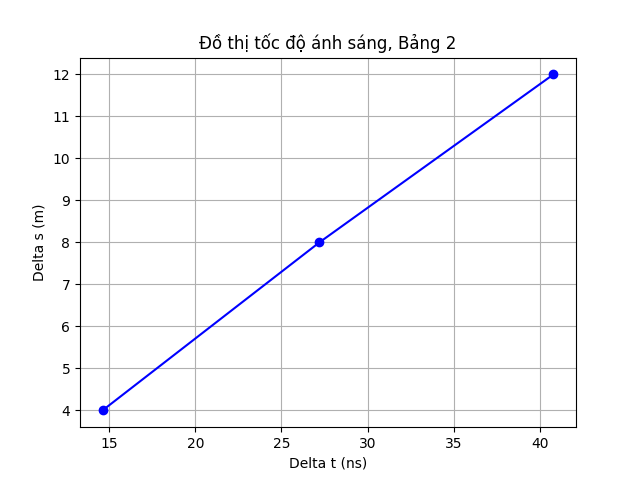
\includegraphics{Figure_1.png}
	\section{Nhận xét}
	Nguyên nhân gây ra sai số
	\begin{itemize}
	    \item Do máy móc và dụng cụ đo thiếu chính xác.
	    \item Do người đo với trình độ tay nghề chưa cao, khả năng các giác quan bị hạn chế
	    \item Do điều kiện ngoại cảnh bên ngoài tác động tới.
	    \item Do người thực hành không thao tác đúng, quan sát không chính xác.
	\end{itemize}
\end{document}
